
%%% Local Variables:
%%% mode: latex
%%% TeX-master: t
%%% End:
\section{数据分析的``武器库''}

\begin{frame}{\textcolor{white}{空白}}

  \begin{columns}
    \begin{column}{.5\textwidth}
      \begin{figure}
        \centering 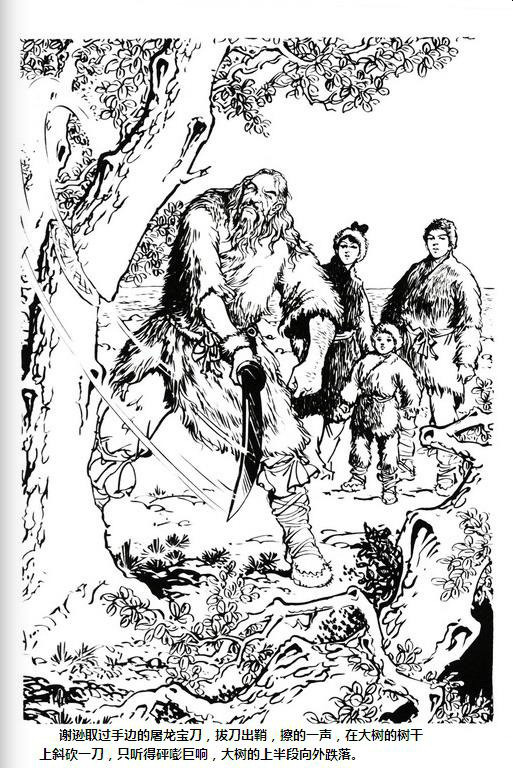
\includegraphics[width=0.95\columnwidth]{chp03_屠龙宝刀.jpg}
      \end{figure}
    \end{column}

    \begin{column}{.5\textwidth}
      \begin{ornamentblock}
        \centering
        {工欲善其事,必先利其器
          \rightline{\textemdash 《论语·卫灵公》}}
      \end{ornamentblock}
    \end{column}
  \end{columns}

\end{frame}

\begin{frame}{数据分析的``七种武器''}
\begin{enumerate}\large
\item 数据采集
\item 数据处理
\item 业务分析
\item 数据建模
\item 数据库
\item 分析算法
\item 可视化
\end{enumerate}
\end{frame}

\subsection{数据采集}
\begin{frame}[t]{\subsecname}
\begin{itemize}
\item<2-> 利用服务器端提供的API接口调取数据
\item<3-> 编写爬虫程序,从网页上抓取数据
\end{itemize}

\begin{overlayarea}{\textwidth}{\textheight}

  \begin{onlyenv}<2>
\begin{table} \centering \scriptsize
  \renewcommand\arraystretch{0.9}
  \begin{tabular}{|m{0.3\columnwidth}|m{0.3\columnwidth}|m{0.3\columnwidth}|}
    \toprule
    \rowcolor{LightCyan}
\multicolumn{1}{|c|}{\textbf{字段名称}} & \multicolumn{1}{c|}{\textbf{字段含义}} & \multicolumn{1}{c|}{\textbf{说明}}\\\hline
     alter & 交通出行方式 & 推荐公交、巴士优先、骑车、小汽车、出租车等 \\\hline
     O\_lon \& O\_lat & 出发地坐标 & 百度公司加密后的经纬度坐标 \\\hline
     D\_lon \& D\_lat & 到达地坐标 & 百度公司加密后的经纬度坐标 \\\hline
     distance & 出行距离 & 包括步行在内的实际路网距离\\\hline
     duration & 出行时间 & 包括步行在内 \\\hline
     price & 票价 & \\\hline
     walkDistance & 步行距离 & \\\hline
     walkTime & 步行时间 & \\\hline
     transferNumber & 换乘次数 & \\    
     \bottomrule
  \end{tabular}
\caption{百度地图API返回的公交路径规划数据结果}
\end{table}
  \end{onlyenv}

\vspace{-15pt}
  \begin{onlyenv}<3>
\begin{figure}
  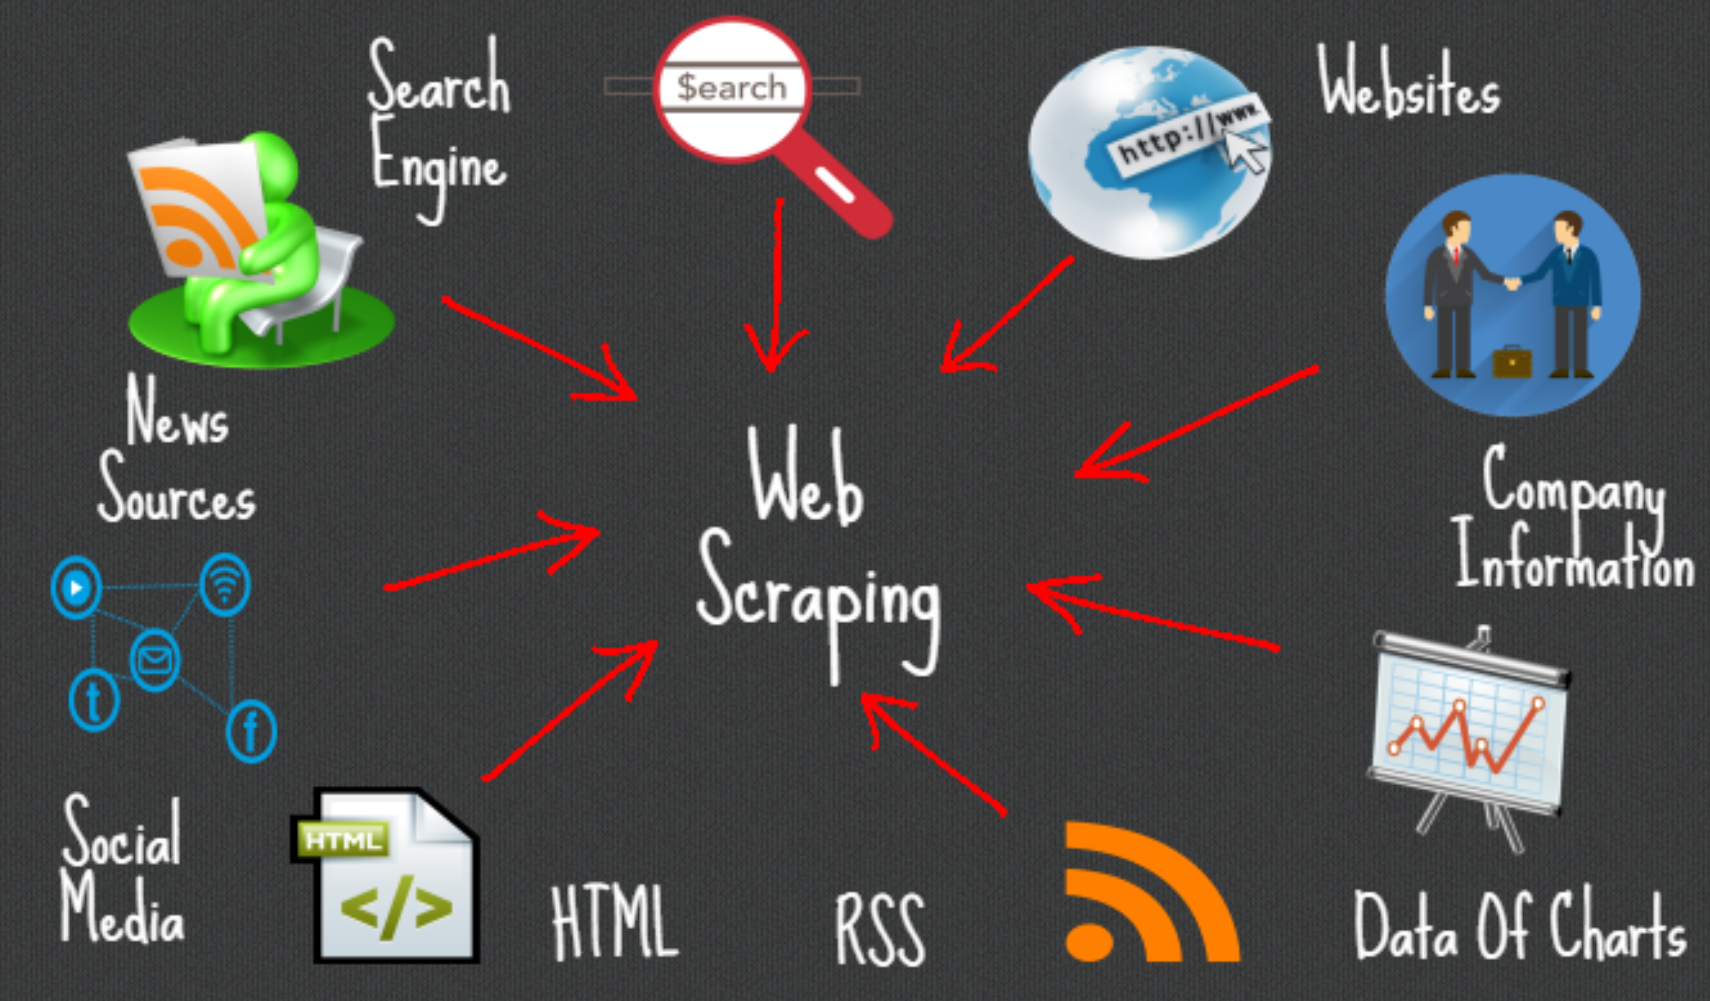
\includegraphics[width=\textwidth]{chp03_网络爬虫.png}
  \caption{利用爬虫程序,可以从丰富的互联网资源中自动化采集数据}
\end{figure}
  \end{onlyenv}
\end{overlayarea}

\end{frame}

\subsection{数据预处理}

\begin{frame}[t]{\subsecname}
\begin{itemize}
\item<1-> 现实中的原始数据都是不完整、不一致的脏数据,需要编写程序对数据进行\emphText{清洗、集成、变换和归约}等自动化处理
\item<2-> 示例:GPS数据预处理
\end{itemize}

\begin{overlayarea}{\textwidth}{\textheight}
  \begin{onlyenv}<2>
\begin{algorithm}[H] \tiny
     \SetKwInOut{Input}{输入}\SetKwInOut{Output}{输出}
     \DontPrintSemicolon 
     \caption*{GPS原始数据清洗}
      
     \KwData{原始车牌GPS文件:GPS\_File,每行$line$=(ID,Postion,Time,Direction,Speed,State)}
     \KwResult{清洗后的GPS文件:GPS\_File\_P}
     \Input{时间容差$\Delta t$, 距离容差$\Delta d$}
     \BlankLine

     \tcc{按行将原始数据读入一个列表$G$}
     \ForEach{$line \in$ GPS\_File}{$G.add(line)$}
     \BlankLine

     \tcc{对$G$按照时间排序}
     SortByTime($G$)
     \BlankLine

     $bFirst$ $\leftarrow$ true

     \For{$i=1 \leftarrow 1$ \KwTo $N$}{
        \lIf{$G[i].position \notin Rect$}{\textbf{continue} \tcc*[r]{剔除位置不在市域范围$Rect$的错误点}} 
        \eIf{$bFirst=true$}{
            GPS\_File\_P $\leftarrow$ OutputResult($G[i]$) \tcc*[r]{输出结果}
            $bFirst \leftarrow$ true\;
            $tt \leftarrow G[i].time$\; 
            $tp \leftarrow G[i].position$\;}
            {
            \tcc{根据前后点时间容差和距离容差剔除错误点}
            \If{$(5 \leqslant (G[i].time-tt) \leqslant{\Delta t}) \cap$
            Distance$(G[i].position,tp) \leqslant \Delta d$}
            {GPS\_File\_P $\leftarrow$ OutputResult($G[i]$) \tcc*[r]{输出结果} 
            $tt \leftarrow G[i].time$\; $tp \leftarrow G[i].position$\;}}
        }
\end{algorithm}
  \end{onlyenv}

  \begin{onlyenv}<3>
\begin{columns}
  \begin{column}{.4\textwidth}
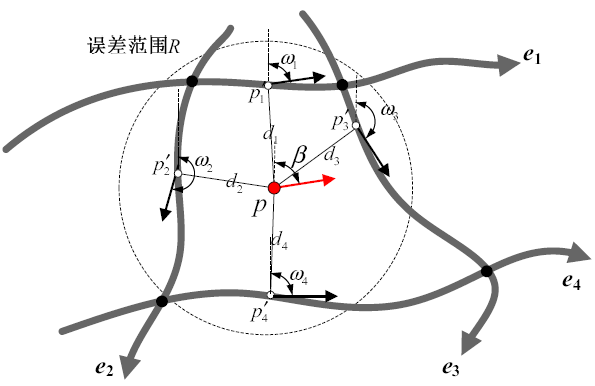
\includegraphics[width=\textwidth]{chp03_地图匹配示意.png}
  \end{column}
  \begin{column}{.6\textwidth}
\begin{algorithm}[H] \tiny
     \SetKwInOut{Input}{输入}\SetKwInOut{Output}{输出}
     \DontPrintSemicolon 
     \caption*{GPS与道路地图匹配}
     \Input{路网模型G和GPS轨迹$T$: $p_1 \rightarrow p_2 \rightarrow \cdots \rightarrow p_n$}
     \Output{处理后的GPS点序列$P$:$c_1^{j_1} \rightarrow c_2^{j_2} \rightarrow \cdots c_n^{j_n}$}
     \BlankLine    
     \tcc{清空列表$tList$}
     $tList \leftarrow empty$ 
     \For{$i = 1$ \KwTo $n$}{
       \tcc{半径r范围内的候选路段集}
       $s$ = GetCandidates($p_i$,$G$,$r$) 
       $tList.add(s)$}
     $G_T^'$ = ConstructGraph($tList$) \tcc*[r]{构建图$G_T^'$}
     return FindMatchedSequence($G_T^'$)
\end{algorithm}
  \end{column}
\end{columns}
  \end{onlyenv}
\end{overlayarea}
\end{frame}

\subsection{业务分析}

\begin{frame}[t]{\subsecname}
\begin{itemize}
\item 数据分析中\emphText{最关键的环节}
\item 结合业务特点,确定待分析的内容和技术路线
\end{itemize}

\begin{figure}
  \centering
  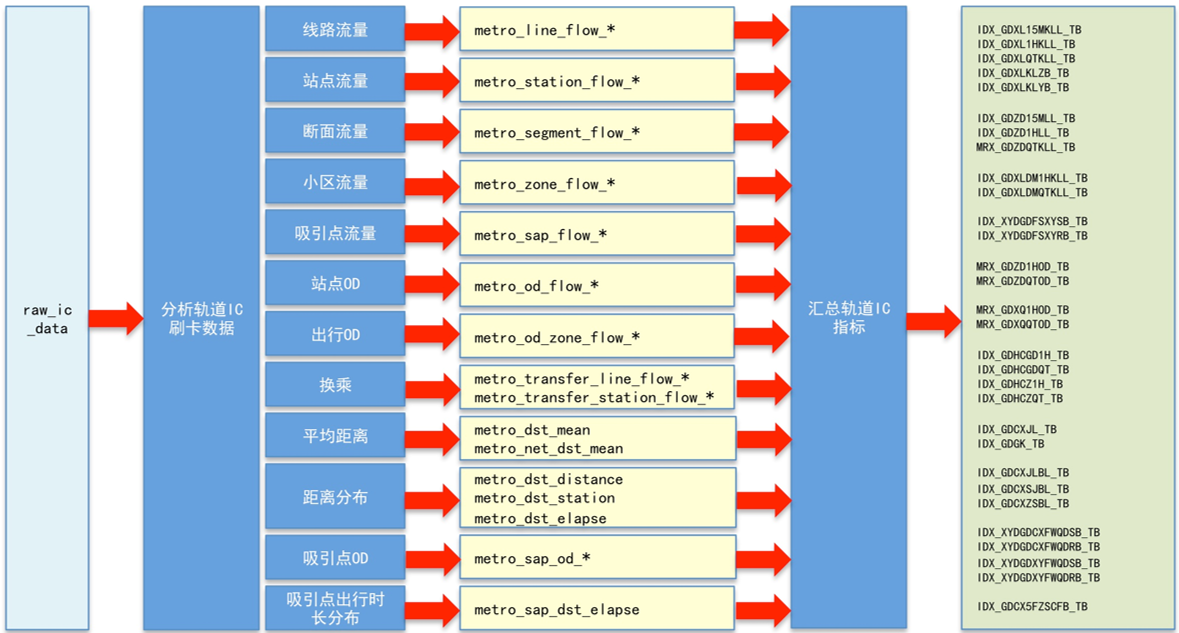
\includegraphics[width=\textwidth]{chp03_轨道刷卡业务分析.png}
  \caption{轨道刷卡数据分析的业务流程}
\end{figure}
\end{frame}

\subsection{数据建模}

\begin{frame}[t]{\subsecname}
\begin{itemize}
\item<1-> \emphText{根据业务需求对数据进行抽象},形成计算机能够理解的逻辑关系和物理结构
\item<2-> 示例:车辆轨迹模型 
\end{itemize}

\begin{overlayarea}{\textwidth}{\textheight}
  \begin{onlyenv}<2>
\begin{figure}
  \centering
  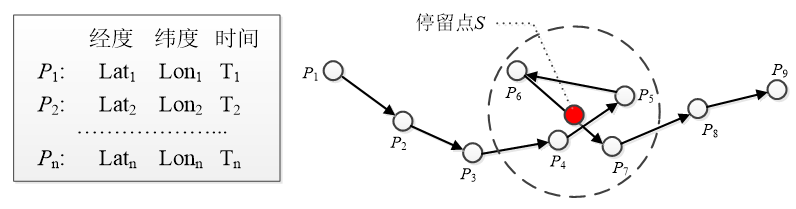
\includegraphics[width=0.8\textwidth]{chp03_停靠点提取算法.png} \\
  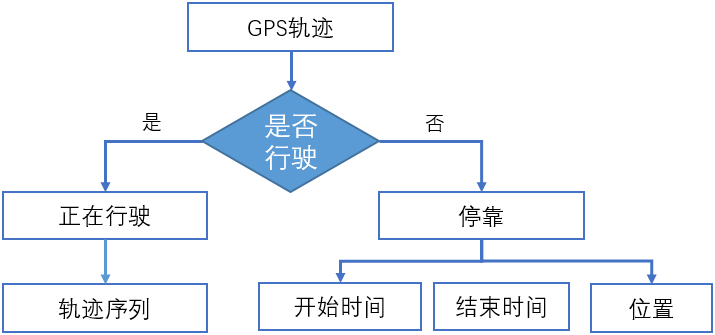
\includegraphics[width=0.6\textwidth]{chp03_GPS轨迹模型.png}
  \caption{车辆轨迹模型}
\end{figure}
  \end{onlyenv}

\vspace{-15pt}
  \begin{onlyenv}<3>
\begin{figure}
  \centering
  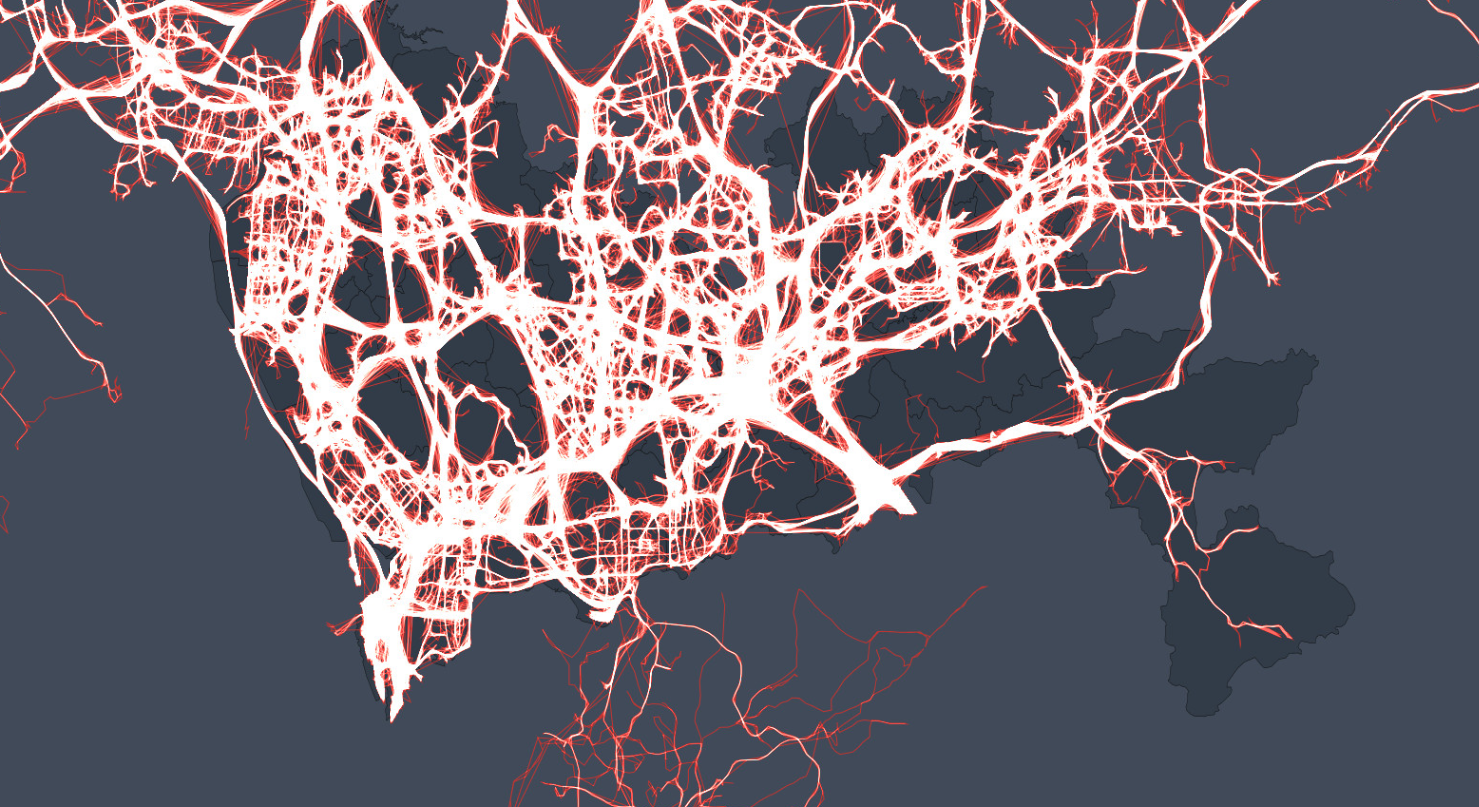
\includegraphics[width=\textwidth]{chp03_车辆轨迹地图.png}
  \caption{车辆轨迹地图}
\end{figure}
  \end{onlyenv}
\end{overlayarea}
\end{frame}

\subsection{数据库}
\begin{frame}[t]{\subsecname}
\begin{itemize}
\item<1-> 通过高效的组织和存储,便于对数据进行新增、删除、修改和查询等操作
\item<2-> 根据数据量级、数据格式选择最适合的数据库技术
\end{itemize}




\subsection{分析算法}
\begin{frame}[t]{\subsecname}
\begin{itemize}
\item<1-> 算法不是简单的数据统计,而是要能够挖掘数据背后的规律和关系
\item<2-> 交通规划中最常用的分析算法是\emphText{空间分析算法}
\end{itemize}

\end{frame}


\subsection{可视化}
\begin{frame}[t]{\subsecname}
\begin{itemize}
\item<1-> 计算机可视化技术与艺术的结合体
\item<2-> 用既直观又简洁的图形来展现分析成果
\end{itemize}

\end{frame}

